\documentclass{exam}
\usepackage[utf8]{inputenc}
\usepackage{lmodern}
\usepackage{microtype}

% \usepackage[parfill]{parskip}
\usepackage[dvipsnames]{xcolor}
\usepackage{amsmath}
\usepackage{amsfonts}
\usepackage{amsthm}
\usepackage{siunitx}
\DeclareSIUnit\year{yr}
\DeclareSIUnit\foot{ft}
\DeclareSIUnit\litre{\liter}

\usepackage{skull}

\usepackage{pgfplots}
\usepgfplotslibrary{polar}
\pgfplotsset{compat=1.11}
\usepgfplotslibrary{statistics}
\usepackage{graphicx}
\usepackage{sidecap}
\sidecaptionvpos{figure}{c}
\usepackage{float}
\usepackage{gensymb}
\usepackage{tkz-euclide}
\usetkzobj{all}
\usepackage{commath}
\usepackage{hyperref}
\usepackage{enumitem}
\usepackage{wasysym}
\usepackage{multicol}
\usepackage{mathtools}
\usepackage{tcolorbox}
\usepackage{tabularx}
\usepackage[version=4]{mhchem}
\usepackage{changepage}
\usepackage{listings}
\lstset{basicstyle=\ttfamily\linespread{0.8}\small}

\renewcommand*{\thefootnote}{\fnsymbol{footnote}}

\newtheorem*{thm}{Theorem}
\newtheorem*{iden}{Identity}
\newtheorem*{lemma}{Lemma}
\newtheorem{obs}{Observation}
\theoremstyle{definition}
\newtheorem*{defn}{Definition}
\newtheorem*{ex}{Example}
\newtheorem{con}{Construction}
\newtheorem*{alg}{Algorithm}

\newtheoremstyle{break}
  {\topsep}{\topsep}%
  {\itshape}{}%
  {\bfseries}{}%
  {\newline}{}%
\theoremstyle{break}
\newtheorem*{bthm}{Theorem}

% russian integral
\usepackage{scalerel}
\DeclareMathOperator*{\rint}{\scalerel*{\rotatebox{17}{$\!\int\!$}}{\int}}

% \DeclareMathOperator*{\rint}{\int}

\pgfplotsset{vasymptote/.style={
    before end axis/.append code={
        \draw[densely dashed] ({rel axis cs:0,0} -| {axis cs:#1,0})
        -- ({rel axis cs:0,1} -| {axis cs:#1,0});
    }
}}

% \pointsinrightmargin
\boxedpoints
\pointname{}

\newcommand{\questioA}{\question[\texttt{\textbf{\color{Cerulean} A}}]}
\newcommand{\questioM}{\question[\texttt{\textbf{\color{PineGreen} M}}]}
\newcommand{\questioE}{\question[\texttt{\textbf{\color{WildStrawberry} E}}]}
\newcommand{\questioS}{\question[\texttt{\textbf{\color{Goldenrod} S}}]}
\newcommand{\questioO}{\question[\texttt{\textbf{\color{BurntOrange} O}}]}

\newcommand{\parA}{\part[\texttt{\textbf{\color{Cerulean} A}}]}
\newcommand{\parM}{\part[\texttt{\textbf{\color{PineGreen} M}}]}
\newcommand{\parE}{\part[\texttt{\textbf{\color{WildStrawberry} E}}]}
\newcommand{\parS}{\part[\texttt{\textbf{\color{Goldenrod} S}}]}
\newcommand{\parO}{\part[\texttt{\textbf{\color{BurntOrange} O}}]}

\newcommand{\subparA}{\subpart[\texttt{\textbf{\color{Cerulean} A}}]}
\newcommand{\subparM}{\subpart[\texttt{\textbf{\color{PineGreen} M}}]}
\newcommand{\subparE}{\subpart[\texttt{\textbf{\color{WildStrawberry} E}}]}
\newcommand{\subparS}{\subpart[\texttt{\textbf{\color{Goldenrod} S}}]}
\newcommand{\subparO}{\subpart[\texttt{\textbf{\color{BurntOrange} O}}]}

\newcommand{\mainHeader}[2]{\section*{NCEA Level 2 Mathematics\\#1. #2}}
\newcommand{\mainHeaderHw}[2]{\section*{NCEA Level 2 Mathematics (Homework)\\#1. #2}}
\newcommand{\seealso}[1]{\begin{center}\emph{See also #1.}\end{center}}
\newcommand{\drills}[1]{\begin{center}\emph{Drill problems: #1.}\end{center}}
\newcommand{\basedon}[1]{\begin{center}\emph{Notes largely based on #1.}\end{center}}


\usepackage{tikzsymbols}

\begin{document}

\section*{NCEA Level 3 Calculus\\Solutions to Homeworks}

\subsection*{1. The Derivative}
\begin{enumerate}
  \item Green: derivative of function. Red: original function.
        \begin{center}
          \fbox{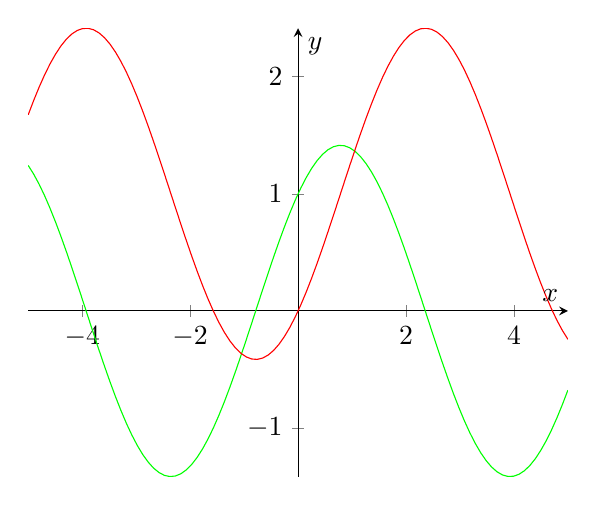
\begin{tikzpicture}
            \begin{axis}[
              axis lines = center,
              xlabel = $ x $,
              ylabel = $ y $
            ]
              \addplot[domain = -5:5, color = green, samples=100] {sin(deg(x)) + cos(deg(x))};
              \addplot[domain = -5:5, color = red, samples=100] {sin(deg(x)) - cos(deg(x)) + 1};
            \end{axis}
          \end{tikzpicture}}
        \end{center}
  \item
    \begin{enumerate}
      \item At a min or max, the function is momentarily horizontal and so has slope zero; so $ m = 0 $.
      \item Consider a graph like the following at $ (0,0) $:
        \begin{center}
          \fbox{\begin{tikzpicture}
            \begin{axis}[
              axis lines = center,
              xlabel = $ x $,
              ylabel = $ y $
            ]
              \addplot[domain = -5:5, color = green, samples=100] {x^3};
            \end{axis}
          \end{tikzpicture}}
        \end{center}
    \end{enumerate}
\end{enumerate}

\subsection*{2. Limits}
\begin{enumerate}
  \item Increasing: the graph of the function is sloping up (green). Decreasing: the graph of the function is sloping down (red). Concave up: the graph
        of the function is increasing in slope (it is like a cup $ \cup $) (blue). Concave down: the graph of the function is decreasing in slope
        (it is like a cap $ \cap $) (orange). Continuous: the function has no holes (all of them except pink).
        \begin{center}
          \fbox{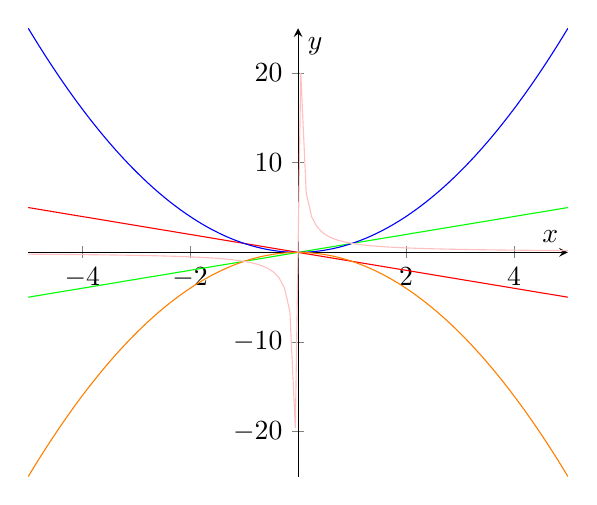
\begin{tikzpicture}
            \begin{axis}[
              axis lines = center,
              xlabel = $ x $,
              ylabel = $ y $
            ]
              \addplot[domain = -5:5, color = green, samples=100] {x};
              \addplot[domain = -5:5, color = red, samples=100] {-x};
              \addplot[domain = -5:5, color = blue, samples=100] {x^2};
              \addplot[domain = -5:5, color = orange, samples=100] {-x^2};
              \addplot[domain = -5:5, color = pink, samples=100] {1/x};
            \end{axis}
          \end{tikzpicture}}
        \end{center}
  \item
    \begin{enumerate}
      \item $ \lim_{x \to -2} f(x) = 0 $, $ \lim_{x \to 2} f(x) = -0.5 $.
      \item No, it approaches different values from the left and the right.
      \item Yes, because the function is continuous there.
      \item $ (-\infty, -3) $, $ (-3, -1) $, $ (-1, 2) $, $ (2, \infty) $.
      \item -3, -1, 2.
    \end{enumerate}
  \item For example,

    \begin{center}
      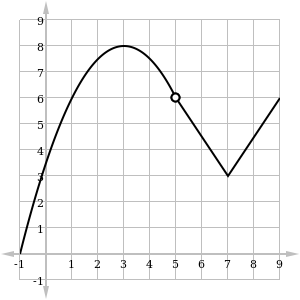
\includegraphics[width=0.4\textwidth]{function}
    \end{center}
\end{enumerate}

\subsection*{3. Derivatives of Common Functions}
\begin{enumerate}
  \item
    \begin{enumerate}
      \item $ 2x + 1/x $
      \item $ t^2 x^{t - 1} $
      \item $ \cos x + \sin x $
      \item $ \frac{4}{5} x^{-1/5} = \dfrac{4}{5 \sqrt[5]{x}} $
    \end{enumerate}
  \item The power $ x $ is not constant.
  \item Consider $ x^{-n} $. The first derivative is $ -n x^{-n - 1} $, the second is $ n(n+1) x^{-n - 2} $, and so the $ n$th
        is $ (-1)^n n(n+1)\cdots(2n - 1)(2n) x^{-2n} = (-1)^n \frac{(2n)!}{(n-1)!} x^{-2n} $. [This can be proved via induction.]
  \item
    \begin{enumerate}
      \item Note first that $ 10^t = e^{t \ln 10} $, so $ P = P_0 + e^{t \ln 10} $ and $ \od{P}{t} = (\ln 10)e^{t \ln 10} = (\ln 10)10^t $.
            At $ t = 100 $, we have $ \od{P}{t} = \num{2.3e100} $.
      \item Real-world populations don't grow exponentially forever if there are finite resources (e.g. food).
    \end{enumerate}
\end{enumerate}

\subsection*{4. The Chain Rule}
\begin{enumerate}
  \item $ \od{y}{x} = \frac{-\csc^2 x}{2\sqrt{\cot x}} $
  \item
    \begin{enumerate}
      \item Simply apply the chain rule twice.
      \item $ y' = 5x^4 (\cos x^5)(-\sin \sin x^5)(\cos \cos \sin x^5)(-\sin \sin \cos \sin x^5)(\cos \cos \sin \cos \sin x^5) $.
    \end{enumerate}
  \item
    \begin{enumerate}
      \item $ f'(\theta) = -2 \sin 2\theta $ and $ g'(\theta) = -4\sin \theta \cos \theta = -2\sin 2\theta $, so $ f' = g' $ as they agree everywhere.
      \item Since $ f $ and $ g $ have the same derivative, they differ only by a constant. But $ f(0) = 1 = g(0) $, so that constant is zero; hence $ f = g $.
    \end{enumerate}
\end{enumerate}

\subsection*{5. The Product and Quotient Rules}
\begin{enumerate}
  \item
    \begin{enumerate}
      \item $ \cos x \ln x + \dfrac{\sin x}{x} $
      \item $ \sec kx + kx \sec kx \tan kx $
      \item $ \dfrac{-\pi(\sin \pi \theta + \cos \pi \theta)\sin \pi \theta - \pi(\cos \pi \theta - \sin \pi \theta) \cos \pi \theta}{(\sin \pi \theta + \cos \pi \theta)^2} $
      \item $ (\cos t)(3\sin^2 t)(-\sin(\sin^3 t))(4 \cos^3 \sin^3 t) $.
    \end{enumerate}
  \item
    \begin{align*}
      F = \dod{}{t} \frac{m_0 v}{\sqrt{1 - \dfrac{v^2}{c^2}}} &= a \dod{}{v} \frac{m_0 v}{\sqrt{1 - \dfrac{v^2}{c^2}}}\\
       &= a \left(\frac{m_0}{\sqrt{1 - \dfrac{v^2}{c^2}}} + \frac{m_0 v^2}{c^2\left(1 - \dfrac{v^2}{c^2}\right)^{3/2}} \right)\\
       &= a \left(\frac{m_0 c^2 \left(1 - \dfrac{v^2}{c^2}\right)}{c^2\left(1 - \dfrac{v^2}{c^2}\right)^{3/2}} + \frac{m_0 v^2}{c^2\left(1 - \dfrac{v^2}{c^2}\right)^{3/2}} \right)\\
       &= m_0 a \left(\frac{c^2 \left(1 - \dfrac{v^2}{c^2}\right) + v^2}{c^2\left(1 - \dfrac{v^2}{c^2}\right)^{3/2}} \right)\\
       &= m_0 a \left(\frac{c^2 - v^2 + v^2}{c^2\left(1 - \dfrac{v^2}{c^2}\right)^{3/2}} \right)\\
       &= \frac{m_0 a}{\left(1 - \dfrac{v^2}{c^2}\right)^{3/2}}.
    \end{align*}
  \item We wish to find $ \od{}{\theta} \sin{\mathrm{rad}(\theta)} $, where $ \mathrm{rad}(\theta) = \frac{\pi \theta}{180} $;
        so $ \od{(\mathrm{rad})}{\theta} = \frac{\pi}{180} $ and $ \od{}{\theta} \sin{\mathrm{rad}(\theta)} = \frac{\pi \theta}{180}\cos{\mathrm{rad}(\theta)} $. [The reason we have to do this is that the derivative of $ \sin $ uses the limit $ \lim_{x \to 0} \frac{\sin x}{x} = 1 $ which
        is false if $ x $ is in degrees.]
\end{enumerate}

\subsection*{6. Tangent and Normal Lines}
\begin{enumerate}
  \item The normal to a curve $ f $ at a point $ (x_0, f(x_0)) $ is the unique line passing through that point that
        is perpendicular to the tangent line of $ f $ at that point.
  \item $ y' = \frac{-\sin(x + \pi)}{2\sqrt{\cos(x + \pi)}} + \cos x - 4\sec x \tan^2 x e^{2\tan^2 x} $; at $ x = \pi $, $ y' = -1 $
        and so the tangent line (best linear approximation) is $ y = -(x - \pi) = \pi - x $.
  \item Since the normal line has slope 3, the tangent line has slope $ -1/3 $. We can take any curve through $ (1,0) $ with this slope,
        so we may as well take the tangent line itself: $ y = -\frac{1}{3}(x - 1) = \frac{1}{3} -\frac{1}{3}x $.
  \item $ \od{y}{x} = \frac{1}{(1 + 3x)^{2/3}} $ and at $ x = 0 $ the slope becomes 1. So the best linear approximation around the point $ (0, 1) $
        is just $ \tilde y = x + 1 $. So at $ x = 0.01, $ we have $ \tilde y = 1.01 $ as our approximate value of $ \sqrt[3]{1.03} $. [The true value
        is around 1.0099, so we are not too far off.]
\end{enumerate}

\subsection*{7. Higher Derivatives and the Geometry of a Function}
\begin{enumerate}
  \item The second derivative tells us the concavity of a function: if the second derivative is positive, the function is curving up
        and if it is negative then the function is curving down.
  \item
    \begin{enumerate}
      \item $ f'(x) = 5x^4 - 5 $, $ f''(x) = 20x^3 $.
      \item $ f'(x) = \frac{x^2 - 2x}{(x - 1)^2} $, $ f''(x) = \frac{2x - 2}{(x - 1)^4} $.
      \item $ f'(x) = \frac{1}{2} x^{-1/2} - \frac{1}{4} x^{-3/4} $,
            $ f''(x) = -\frac{1}{4} x^{-3/2} + \frac{3}{16}x^{-5/4} = \frac{3}{16\sqrt[4]{x^5}} - \frac{1}{4\sqrt{x^3}} $.
    \end{enumerate}
  \item
    \begin{enumerate}
      \item For example,

            \begin{center}
              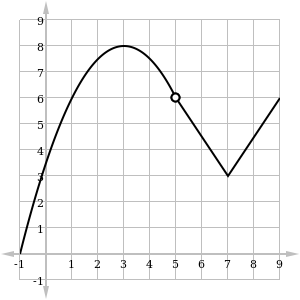
\includegraphics[width=0.4\textwidth]{function}
            \end{center}

      \item For example,

        \begin{center}
          \fbox{\begin{tikzpicture}
            \begin{axis}[
              axis lines = center,
              xlabel = $ x $,
              ylabel = $ y $
            ]
              \addplot[domain = -5:5, color = green, samples=100] {-exp(x) + 50};
            \end{axis}
          \end{tikzpicture}}
        \end{center}

    \end{enumerate}
\end{enumerate}

\subsection*{8. Optimisation}
\begin{enumerate}
  \item At some point $ x $, the distance between the two parabolae is $ \delta(x) = (x^2 + 1) - (x - x^2) = 2x^2 - x + 1 $. Taking
        the derivative, we find $ \delta'(x) = 4x - 1 $ which has a single zero at $ x = 1/4 $; by looking at the graph of the two
        parabolae, we see that this must be the location of the miniumum distance $ \delta(1/4) = 7/8 $ units.
  \item If $ y = 3x + 2\cos x + 5 $, then $ \od{y}{x} = 3 -2\sin x $. Since $ 1 \geq \sin x $, $ 3 - 2\sin x \geq 1 $. In particular,
        the function is everywhere increasing. Now, note that when $ x = -200\pi $, $ y = -600\pi + 7 < 0 $, and when $ x = 200\pi $,
        $ y = 600\pi + 7 > 0 $. Since the function is continuous over this interval, it follows that at some point it passes through
        the $ y$-axis and has at least one root; since it is increasing everywhere, it must have exactly one real root.
  \item The area of such a rectangle will be $ A = 4x b\sqrt{1 - \frac{x^2}{a^2}} $; so
        \begin{displaymath}
          \od{A}{x} = 4b\sqrt{1 - \frac{x^2}{a^2}} - \frac{4x^2b}{a^2\sqrt{1 - \frac{x^2}{a^2}}}.
        \end{displaymath}
        Setting this to zero, we have $ a^2 = 2x^2 $ and so $ 2x = \sqrt{2}a $. It follows that $ 2y = b\sqrt{2} $, and so the maximal
        area is $ 2ab $.
  \item Consider the following diagram.
        \begin{center}
          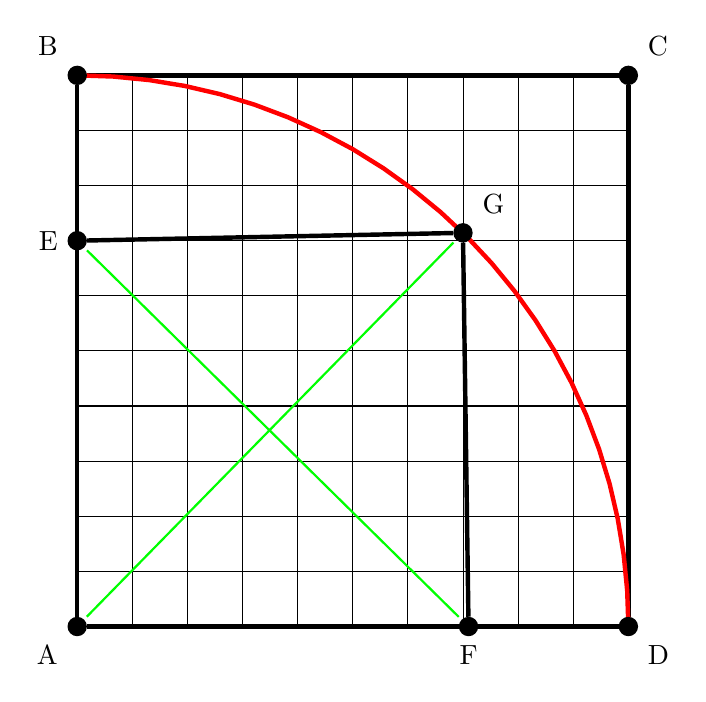
\begin{tikzpicture}[scale=7]
            \draw[step=0.1,black,thin] (0,0) grid (1,1);
            \node[label=below left:A] (A) at (0,0) {};
            \node[label=above left:B] (B) at (0,1) {};
            \node[label=above right:C] (C) at (1,1) {};
            \node[label=below right:D] (D) at (1,0) {};
            \node[label=left:E] (E) at (0,0.7) {};
            \node[label=below:F] (F) at (0.71,0) {};
            \node[label=above right:G] (G) at (0.6999,0.7143) {};
            \draw[ultra thick] (A) -- (B) -- (C) -- (D) -- (A);
            \draw[ultra thick] (E) -- (G) -- (F);
            \draw[thick, green] (A) -- (G);
            \draw[thick, green] (E) -- (F);
            \draw[red,ultra thick,domain=0:90] plot ({cos(\x)}, {sin(\x)});
            \fill (A) circle [radius=0.5pt];
            \fill (B) circle [radius=0.5pt];
            \fill (C) circle [radius=0.5pt];
            \fill (D) circle [radius=0.5pt];
            \fill (E) circle [radius=0.5pt];
            \fill (F) circle [radius=0.5pt];
            \fill (G) circle [radius=0.5pt];
          \end{tikzpicture}
        \end{center}
        It should be clear that $ AG = 1 $; call $ \angle AEG = \theta $ and $ \angle AFG = \phi $, and let $ AE = EG = e $
        and $ AF = GF = f $. By the cosine rule, we have $ 1 = 2e^2  (1 - \cos \theta) $ and $ 1 = 2f^2 (1 - \cos \phi) $. Now,
        the area of the triangle $ \triangle AEG $ is given by $ \frac{1}{2}\sqrt{e^2 - \frac{1}{4}} $; the area of $ \triangle AFG $ is
        given by $ \frac{1}{2}\sqrt{f^2 - \frac{1}{4}} $. Since $ AEFG $ is a (convex) quadrilateral with two right angles, $ \theta + \phi = \pi $.
        Putting this all together, the area of the quadrilateral is $ A = \frac{1}{2}\sqrt{e^2 - \frac{1}{4}} + \frac{1}{2}\sqrt{f^2 - \frac{1}{4}} $. We
        have that $ e^2 = \frac{1}{2(1 - \cos \theta)} $ and $ f^2  = \frac{1}{2(1 - \cos(\pi - \theta))} =\frac{1}{2(1 + \cos(\theta))} $,
        so the area in terms of $ \theta $ is
        \begin{displaymath}
          A = \frac{1}{2}\sqrt{\frac{1}{2(1 - \cos \theta)} - \frac{1}{4}} + \frac{1}{2}\sqrt{\frac{1}{2(1 + \cos \theta)} - \frac{1}{4}}.
        \end{displaymath}
        Taking the derivative, we obtain
        \begin{displaymath}
          \od{A}{\theta} = \frac{1}{2}\frac{\sin \theta}{4(\cos \theta + 1)^2 \sqrt{\frac{1}{2(1 + \cos \theta)} - \frac{1}{4}}}
                         - \frac{1}{2}\frac{\sin \theta}{4(1 - \cos \theta)^2 \sqrt{\frac{1}{2(1 - \cos \theta)} - \frac{1}{4}}};
        \end{displaymath}
        Now we set this to zero. We know that $ 0 < \theta < \pi $, so $ \sin \theta \neq 0 $ and hence
        \begin{gather*}
          4(\cos \theta + 1)^2 \sqrt{\frac{1}{2(1 + \cos \theta)} - \frac{1}{4}}
              = 4(1 - \cos \theta)^2 \sqrt{\frac{1}{2(1 - \cos \theta)} - \frac{1}{4}}\\
          \sqrt{\frac{1}{2} - \frac{\cos \theta + 1}{4}} = \sqrt{\frac{1}{2} - \frac{1 - \cos \theta}{4}}\\
          \cos \theta = - \cos \theta\\
          \cos \theta = 0
        \end{gather*}
        Hence $ \theta = \phi = \pi/2 $. Immediate calculation shows that $ e = f = \frac{1}{\sqrt{2}} $; we thus
        have a square with side length $ 1/\sqrt{2} $, and area $ \frac{1}{2} $. Is this a maximum or a minimum? We
        cheat by graphing the area versus $ \theta $:
        \begin{center}
          \fbox{\begin{tikzpicture}
            \begin{axis}[
              axis lines = center,
              xlabel = $ \theta $,
              ylabel = $ A $,
              ymin = 0,
              ymax = 3
            ]
              \addplot[domain = 0.01:3.14, color = green, samples=100] {0.5*sqrt(1/(2 - 2*cos(deg(x))) - 1/4) + 0.5*sqrt(1/(2 + 2*cos(deg(x))) - 1/4)};
              \addplot[domain = 0.01:3.14, color = red, samples=100] {0.5};
            \end{axis}
          \end{tikzpicture}}
        \end{center}
        so we obviously have the minimum area:
        \begin{center}
          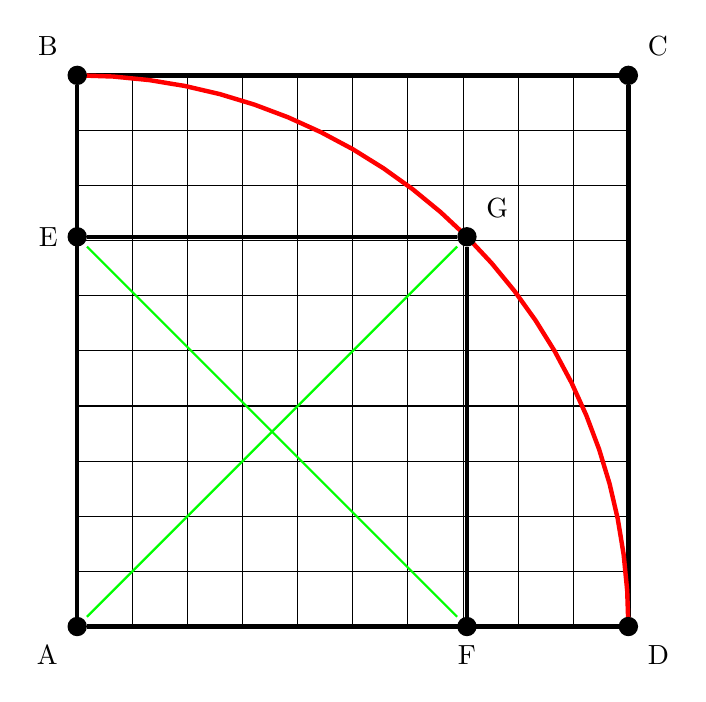
\begin{tikzpicture}[scale=7]
            \draw[step=0.1,black,thin] (0,0) grid (1,1);
            \node[label=below left:A] (A) at (0,0) {};
            \node[label=above left:B] (B) at (0,1) {};
            \node[label=above right:C] (C) at (1,1) {};
            \node[label=below right:D] (D) at (1,0) {};
            \node[label=left:E] (E) at (0,0.7071) {};
            \node[label=below:F] (F) at (0.7071,0) {};
            \node[label=above right:G] (G) at (0.7071,0.7071) {};
            \draw[ultra thick] (A) -- (B) -- (C) -- (D) -- (A);
            \draw[ultra thick] (E) -- (G) -- (F);
            \draw[thick, green] (A) -- (G);
            \draw[thick, green] (E) -- (F);
            \draw[red,ultra thick,domain=0:90] plot ({cos(\x)}, {sin(\x)});
            \fill (A) circle [radius=0.5pt];
            \fill (B) circle [radius=0.5pt];
            \fill (C) circle [radius=0.5pt];
            \fill (D) circle [radius=0.5pt];
            \fill (E) circle [radius=0.5pt];
            \fill (F) circle [radius=0.5pt];
            \fill (G) circle [radius=0.5pt];
          \end{tikzpicture}
        \end{center}

        Note that $ \theta \geq \pi/2 $, because otherwise $ e > 1 $. Suppose we take $ \theta = 2\pi/3 $; here is the graphed figure (with area 1.1547):
        \begin{center}
          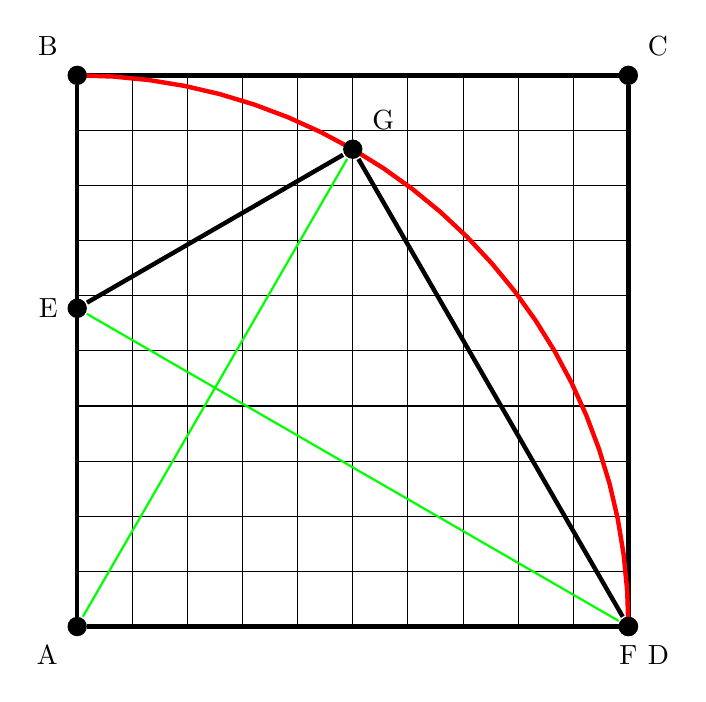
\begin{tikzpicture}[scale=7]
            \draw[step=0.1,black,thin] (0,0) grid (1,1);
            \node[label=below left:A] (A) at (0,0) {};
            \node[label=above left:B] (B) at (0,1) {};
            \node[label=above right:C] (C) at (1,1) {};
            \node[label=below right:D] (D) at (1,0) {};
            \node[label=left:E] (E) at (0,0.5774) {};
            \node[label=below:F] (F) at (1,0) {};
            \node[label=above right:G] (G) at (0.5,0.866) {};
            \draw[ultra thick] (A) -- (B) -- (C) -- (D) -- (A);
            \draw[ultra thick] (E) -- (G) -- (F);
            \draw[thick, green] (A) -- (G);
            \draw[thick, green] (E) -- (F);
            \draw[red,ultra thick,domain=0:90] plot ({cos(\x)}, {sin(\x)});
            \fill (A) circle [radius=0.5pt];
            \fill (B) circle [radius=0.5pt];
            \fill (C) circle [radius=0.5pt];
            \fill (D) circle [radius=0.5pt];
            \fill (E) circle [radius=0.5pt];
            \fill (F) circle [radius=0.5pt];
            \fill (G) circle [radius=0.5pt];
          \end{tikzpicture}
        \end{center}
        This is the maximum area, since if we increase $ \theta $ any more it requires $ f > 1 $.
\end{enumerate}

\subsection*{9. Implicit Differentiation}
\begin{enumerate}
  \item
    \begin{enumerate}
      \item $ y' = \frac{3x^2 + 6x}{2y} $.
      \item $ (1 + y')\sin(x + y) = 2 - 2y' \implies y' = \frac{2 - \sin(x + y)}{2 + \sin(x + y)} $.
      \item $ y' = \frac{20x^3 - 2x}{2y} $.
    \end{enumerate}
  \item $ 2x + 2y + 2xy' - 2yy' + 1 = 0 \implies y' = \frac{-1 - 2x - 2y}{2x - 2y} $, so $ y'(1,2) = \frac{-1 - 2 - 4}{2 - 4} = 7/2 $; hence the
        slope of the normal is $ -2/7 $, and the equation of the normal line is $ y - 2 = -\frac{2}{7}(x - 1) $.
  \item We have $ \frac{1}{2\sqrt{x}} + \frac{1}{2\sqrt{y}} y' = 0 $; suppose we have a tangent line passing through $ (x_0, (\sqrt{c} - \sqrt{x_0})^2) $.
        Then the equation of this tangent is $ y - (\sqrt{c} - \sqrt{x_0})^2 = -\frac{\sqrt{c} - \sqrt{x_0}}{\sqrt{x_0}} (x - x_0) $.
        When $ y = 0 $ we obtain the $ x$-intercept; $ 0 = (\sqrt{c} - \sqrt{x_0})^2 -\frac{\sqrt{c} - \sqrt{x_0}}{\sqrt{x_0}} (x - x_0) $ and so $ x = \sqrt{x_0 c} $.
        Similarly, when $ x = 0 $ we obtain $ y = \sqrt{x_0 c} -  x_0 $. Their sum is therefore $ 2\sqrt{x_0 c} - x_0 = 2\sqrt{c}(\sqrt{c} - \sqrt{y_0}) - (\sqrt{c} - \sqrt{y_0})^2 = c $.
\end{enumerate}

\subsection*{10. Inverse Functions}
\begin{enumerate}
  \item
    \begin{enumerate}
      \item $ y' = \frac{2x}{1+x^4} $.
      \item $ f'(x) = \frac{1}{1+x^2} $.
      \item $ g'(x) = \frac{1}{2\sqrt{x}} \frac{1}{\sqrt{1 - x}} \frac{1}{1+(\sin^{-1} \sqrt{x})^2}  $.
    \end{enumerate}
  \item
    \begin{align*}
      \od{}{x} \left( \frac{1}{2} \tan^{-1} x + \frac{1}{4} \ln\frac{(x + 1)^2}{x^2 + 1} \right)
         &= \frac{1}{2 + 2x^2}  + \frac{1}{4} \frac{x^2 + 1}{(x + 1)^2} \frac{2-2x^2}{(x^2 + 1)^2}\\
         &= \frac{1}{2 + 2x^2}  + \frac{1}{2} \frac{1-x^2}{(x + 1)^2(x^2 + 1)}\\
         &= \frac{1}{2} \frac{(x + 1)^2 + 1 - x^2}{(x + 1)^2 (1 + x^2)}\\
         &= \frac{1}{2} \frac{2x + 2}{(x + 1)^2 (1 + x^2)}\\
         &= \frac{1}{(x + 1)(x^2 + 1)}.
    \end{align*}
  \item Let $ y = \cot^{-1} x $, so that $ x = \cot y $ and $ \od{x}{y} = -\csc^2 y $; hence $ \od{y}{x} = -\sin^2 y $.
        Consider the following triangle:
        \begin{center}
          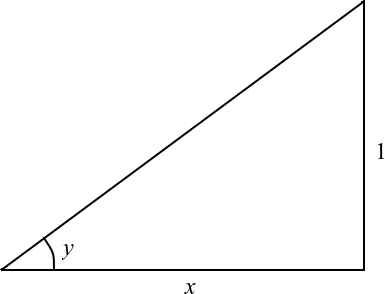
\includegraphics[width=0.3\textwidth]{antitriangle2}
        \end{center}
        So $ \sin y = \frac{1}{\sqrt{1 + x^2}} $, and $ \od{y}{x} = -\frac{1}{1 + x^2} $.
\end{enumerate}

\subsection*{11. Related Rates of Change}
\begin{enumerate}
  \item $ V = [x(t)]^3 $, so $ \od{V}{t} = 3\od{x}{t} [x(t)]^2 $.
  \item The volume of a cone is $ \frac{\pi}{3}r^2 h $. Comparing similar triangles, if the water is at a height $ h $ then it forms a cone
        with radius $ r = h/2 $. Hence when the water is at a height $ h $ it has volume $ V(t) = \frac{\pi [h(t)]^3}{24} $, and
        so $ \od{V}{t} = \frac{\pi [h(t)]^2}{8} \od{h}{t} $. We know that $ \od{V}{t} = 2 $, so solving for $ \od{h}{t} $ we have
        that $ \od{h}{t} = \frac{16}{\pi [h(t)]^2} $ and when $ h = 3 $ the height is rising at a rate of \SI{0.57}{\metre\per\minute}.
  \item Let $ x $ be the hypotenuse of the formed triangle, and let $ y $ be the horizontal distance from the boat to the jetty
        so that $ y = \sqrt{x^2 - 1} $. Then $ \od{y}{t} = \frac{x}{\sqrt{x^2 - 1}} \od{x}{t} = \frac{\sqrt{y^2 + 1}}{y} $. So
        at $ y = 8 $, $ \od{y}{t} = \frac{\sqrt{65}}{8} \approx \SI{1.0078}{\metre\per\second} $.
\end{enumerate}

\subsection*{12. Parametric Functions}
\begin{enumerate}
  \item
    \begin{enumerate}
      \item $ \od{x}{t} = 4t^3 - 6t^2 + 4t $, $ \od{y}{t} = 3t^2 - 1 $, $ \od{y}{x} = \frac{3t^2 - 1}{4t^3 - 6t^2 + 4t} $,
            $ \od[2]{y}{x} = -\frac{3 t^4-6 t^2+3 t-1}{(4t^3 - 6t^2 + 4t)t^2 {\left(2 t^2-3 t+2\right)}^2} $.
      \item $ \od{x}{t} = -\sin t - 4\sin 2t $, $ \od{y}{t} = \cos t + 4\cos 2t $, $ \od{y}{x} = -\frac{\cos t + 4\cos 2t}{\sin t + 4\sin 2t} $,
            $ \od[2]{y}{x} = \frac{12 \cos\left(t\right)+33}{ (\sin t - 4\sin 2t) {\left(8 \cos\left(t\right)+1\right)}^2 \left({\cos\left(t\right)}^2-1\right)} $
    \end{enumerate}
  \item We have $ t^2 = (x - 1)^2 $, so $ y = e^{(x - 1)^2} $ and $ \od{y}{x} = 2(x-1) e^{(x-1)^2} $. At $ x = 2 $, $ \od{y}{x} = 2e $; so the
        best linear approximation is $ y - e = 2e(x - 2) $, or $ y =  e(2x - 3) $.
  \item
    \begin{enumerate}
      \item Should look something like this:

            \begin{center}
              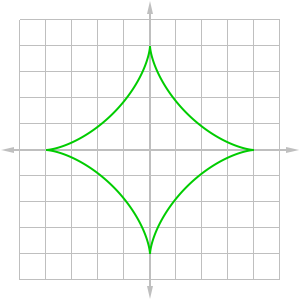
\includegraphics[width=0.4\textwidth]{astroid}
            \end{center}
      \item $ \od{x}{t} = -12\sin t \cos^2 t $, $ \od{y}{t} = 12\cos t \sin^2 t $, so the slope at some $ t $ is simply
            \begin{displaymath}
              \od{y}{x} = \frac{12\cos t \sin^2 t}{-12\sin t \cos^2 t} = -\frac{\sin t}{\cos t}.
            \end{displaymath}
      \item Cusps will be at precisely those points with turning points in the $ x $ or $ y $ direction (for $ 0 \leq t \leq 2\pi $). In
            other words, places where either $ \sin t $ or $ \cos t $ vanishes. These are at $ t \in \left\{0, \frac{\pi}{2}, \pi, \frac{3\pi}{2}, 2\pi\right\} $;
            substituting these into the equation gives us the four points $ (\pm 4, 0) $ and $ (0, \pm 4) $.
    \end{enumerate}
\end{enumerate}


\subsection*{13. Sequences and Series}
\begin{enumerate}
  \item
    \begin{enumerate}
      \item Converges to $1/2$.
      \item Diverges: $ 9^{n + 1}/10^n = 9^{n + 1}/(9 + 1)^n = 9^{n + 1}/(9^n + \cdots) \to \infty $.
    \end{enumerate}
  \item
    \begin{enumerate}
      \item The series is $ 2/3 - 2/5 + 2/7 - 2/9 + \cdots $. It has partial sums $ 2/3,4/15,58/105, \dots $. Converges to $ \pi/2 $.
      \item The series is $ -2/5 + 4/6 - 6/7 + 8/8 - 10/9 + \cdots $. It has partial sums $ 4/15,-62/125, \dots $. Diverges (the terms added and subtracted
            keep growing, so partial sums become very positive and very negative alternately).
    \end{enumerate}
\end{enumerate}

\subsection*{14. Differentiation Revision}
\begin{enumerate}
  \item
    \begin{enumerate}
      \item $ f'(x) = (2017 \times 3)x^{2016} - \frac{1}{19x^{20}} + \frac{1}{2017 \sqrt[2017]{(x + 2)^{2016}}} $.
      \item $ f'(h) = \pi r^2 $.
      \item $ f'(\theta) = -\frac{\mu m g (\mu \cos \theta - \sin \theta)}{(\mu \sin \theta + \cos \theta)^2} $.
      \item $ f'(g) = \frac{(g^2 + \ln g)\cos g - (2g + 1/g)\sin g}{(g^2 + \ln g)^2} $.
      \item $ 3f(x) + 3xf'(x) + 2f(x) f'(x) = \frac{3 + f(x) - xf'(x)}{[3 + f(x)]^2} $
            so $ f'(x) = \frac{3 + f(x) - 3[3 + f(x)]^2f(x)}{3[3 + f(x)]^2x + 2[3 + f(x)]^2f(x) + x} $.
    \end{enumerate}
  \item Let $ \theta $ between the angle of the kite string, and let $ x $ be the horizontal distance to the kite along the ground (so the
        length of the string is $ \sqrt{50^2 + x^2} $). Then $ \sin \theta = 50/x $, so $ \cos \theta \od{\theta}{t} = -\frac{50}{x^2} \od{x}{t} $.
        When the length of the string is 100, $ x \approx 86.6 $; so $ \cos \theta = x/100 \approx 0.866 $. Substituting $ \od{x}{t} = 2 $, we have
        $ \od{\theta}{t} = -\frac{100}{86.6^2} \cdot \frac{1}{0.866} = -0.0154 $.
  \item The surface area of a cone is $ \mathcal{S} = \pi r \sqrt{h^2 + r^2} $; we also have $ 27 = \frac{1}{3} \pi r^2 h $,
        so $ r^2 = \frac{81}{\pi h} $ and
        \begin{gather*}
          \mathcal{S} = \pi \sqrt{\frac{81}{\pi h}\left(h^2 + \frac{81}{\pi h}\right)} = \pi \sqrt{\frac{81h}{\pi} + \frac{81^2}{\pi^2 h^2}}\\
          \od{\mathcal{S}}{h} = \frac{\pi \left( \frac{81}{\pi} - 2\frac{81^2}{\pi^2 h^3} \right) }{2\sqrt{\frac{81h}{\pi} + \frac{81^2}{\pi^2 h^2}}}
        \end{gather*}
        In order to find a minimum, we set this derivative to zero and obtain $ 0 = \frac{81}{\pi} - 2\frac{81^2}{\pi^2 h^3} $, so
        \begin{displaymath}
          h = \sqrt[3]{ 2\frac{81}{\pi} } \approx \SI{3.722}{\centi\metre}.
        \end{displaymath}
        From this, we find $ r = \sqrt{81/\pi h} = \SI{2.63}{\centi\metre} $.
  \item We begin by parameterising the hyperbola; completing the square, we can transform our equation into standard form:
        \begin{displaymath}
          \frac{(x - 1)^2}{3}  - \frac{y^2}{3} = 1
        \end{displaymath}
        A parameterisation of this is $ (1 + \sqrt{3} \sec t, \sqrt{3} \tan t) $. Now, given any point $ (x_0, y_0) $ we wish
        to minimise $ \mathcal{D}(t) = \sqrt{(x_0 - 1 - \sqrt{3} \sec t)^2 + (y_0 - \sqrt{3} \tan t)^2} $ with respect to $ t $.

        \begin{enumerate}
          \item Firstly, consider $ (x_0, y_0) = (2,1) $. Then $ \mathcal{D}(t) = \sqrt{(1 - \sqrt{3}\sec t)^2 + (1 - \sqrt{3} \tan t)^2} $.
                Taking the derivative, we find that:
                \begin{displaymath}
                  \od{\mathcal{D}}{t} = \frac{(\sqrt{3}\sec t - 1)(\sqrt{3}\sec t \tan t) + (\sqrt{3}\tan t - 1)(\sqrt{3}\sec^2 t)}{\sqrt{(1 - \sqrt{3}\sec t)^2 + (1 - \sqrt{3} \tan t)^2}}
                \end{displaymath}
                Using MATLAB to compute the solution of $ \od{\mathcal{D}}{t} = 0 $,
                \begin{center}
                  \verb|vpasolve((sqrt(3) * sec(t) - 1)*(sqrt(3) * sec(t) * tan(t))|\\
                  \qquad\verb|== (1 - sqrt(3)*tan(t))*(sqrt(3)*(sec(t))^2),t)|
                \end{center}
                we find $ t \approx 0.3759 $; so $ (x, y) = (2.8621, 0.6835) $.
            \item Note that $ (3,1) $ is already on the hyperbola. \Innocey
        \end{enumerate}
\end{enumerate}

\subsection*{15. Approximating Areas}
\begin{enumerate}
  \item I use Simpson's rule with $ n = 8 $:
        \begin{displaymath}
          \rint^{1.6}_0 g(x) \dif{x} \approx \frac{0.2}{3} (12.1 + 13.2 + 4(11.6 + 11.1 + 12.2 + 13.0) + 2(11.3 + 11.7 + 12.6)) = 19.21.
        \end{displaymath}
  \item Measure the height of the shaded area at each point (using $ n = 10 $ is probably easiest), collapsing the empty area down (e.g. the height
        of the function at $ x = -1 $ is just $ 3 + 1 = 4 $). Then use some numerical integration method.
  \item Like 2. but simpler.
\end{enumerate}

\subsection*{16. Anti-differentiation}
\begin{enumerate}
  \item
    \begin{enumerate}
      \item $ F(x) = \frac{1}{2}x^2 - 3x + C $
      \item $ f(x) = x^2 + 3x + 2 $, so $ F(x) = \frac{1}{3}x^3 + \frac{3}{2}x^2 + 2x + C $
      \item $ F(\theta) = 2\theta^3 - 7\tan \theta + C $
      \item $ G(h) = \pi^2 h$
      \item $ F(x) = \frac{x^{4.7}}{4.7} + \frac{2}{3} \sqrt{x^3} + \sqrt{7}x^{\sqrt{7}} $
    \end{enumerate}
  \item $ \varphi(x) = x^2 + x + C $; but $ \varphi(1) = 6 $, so $ 1 + 1 + C = 6 $ and $ C = 4 $. Hence $ \varphi(x) = x^2 + x + 4 $, and $ \varphi(2) = 10 $.
  \item See following image.
        \begin{center}
          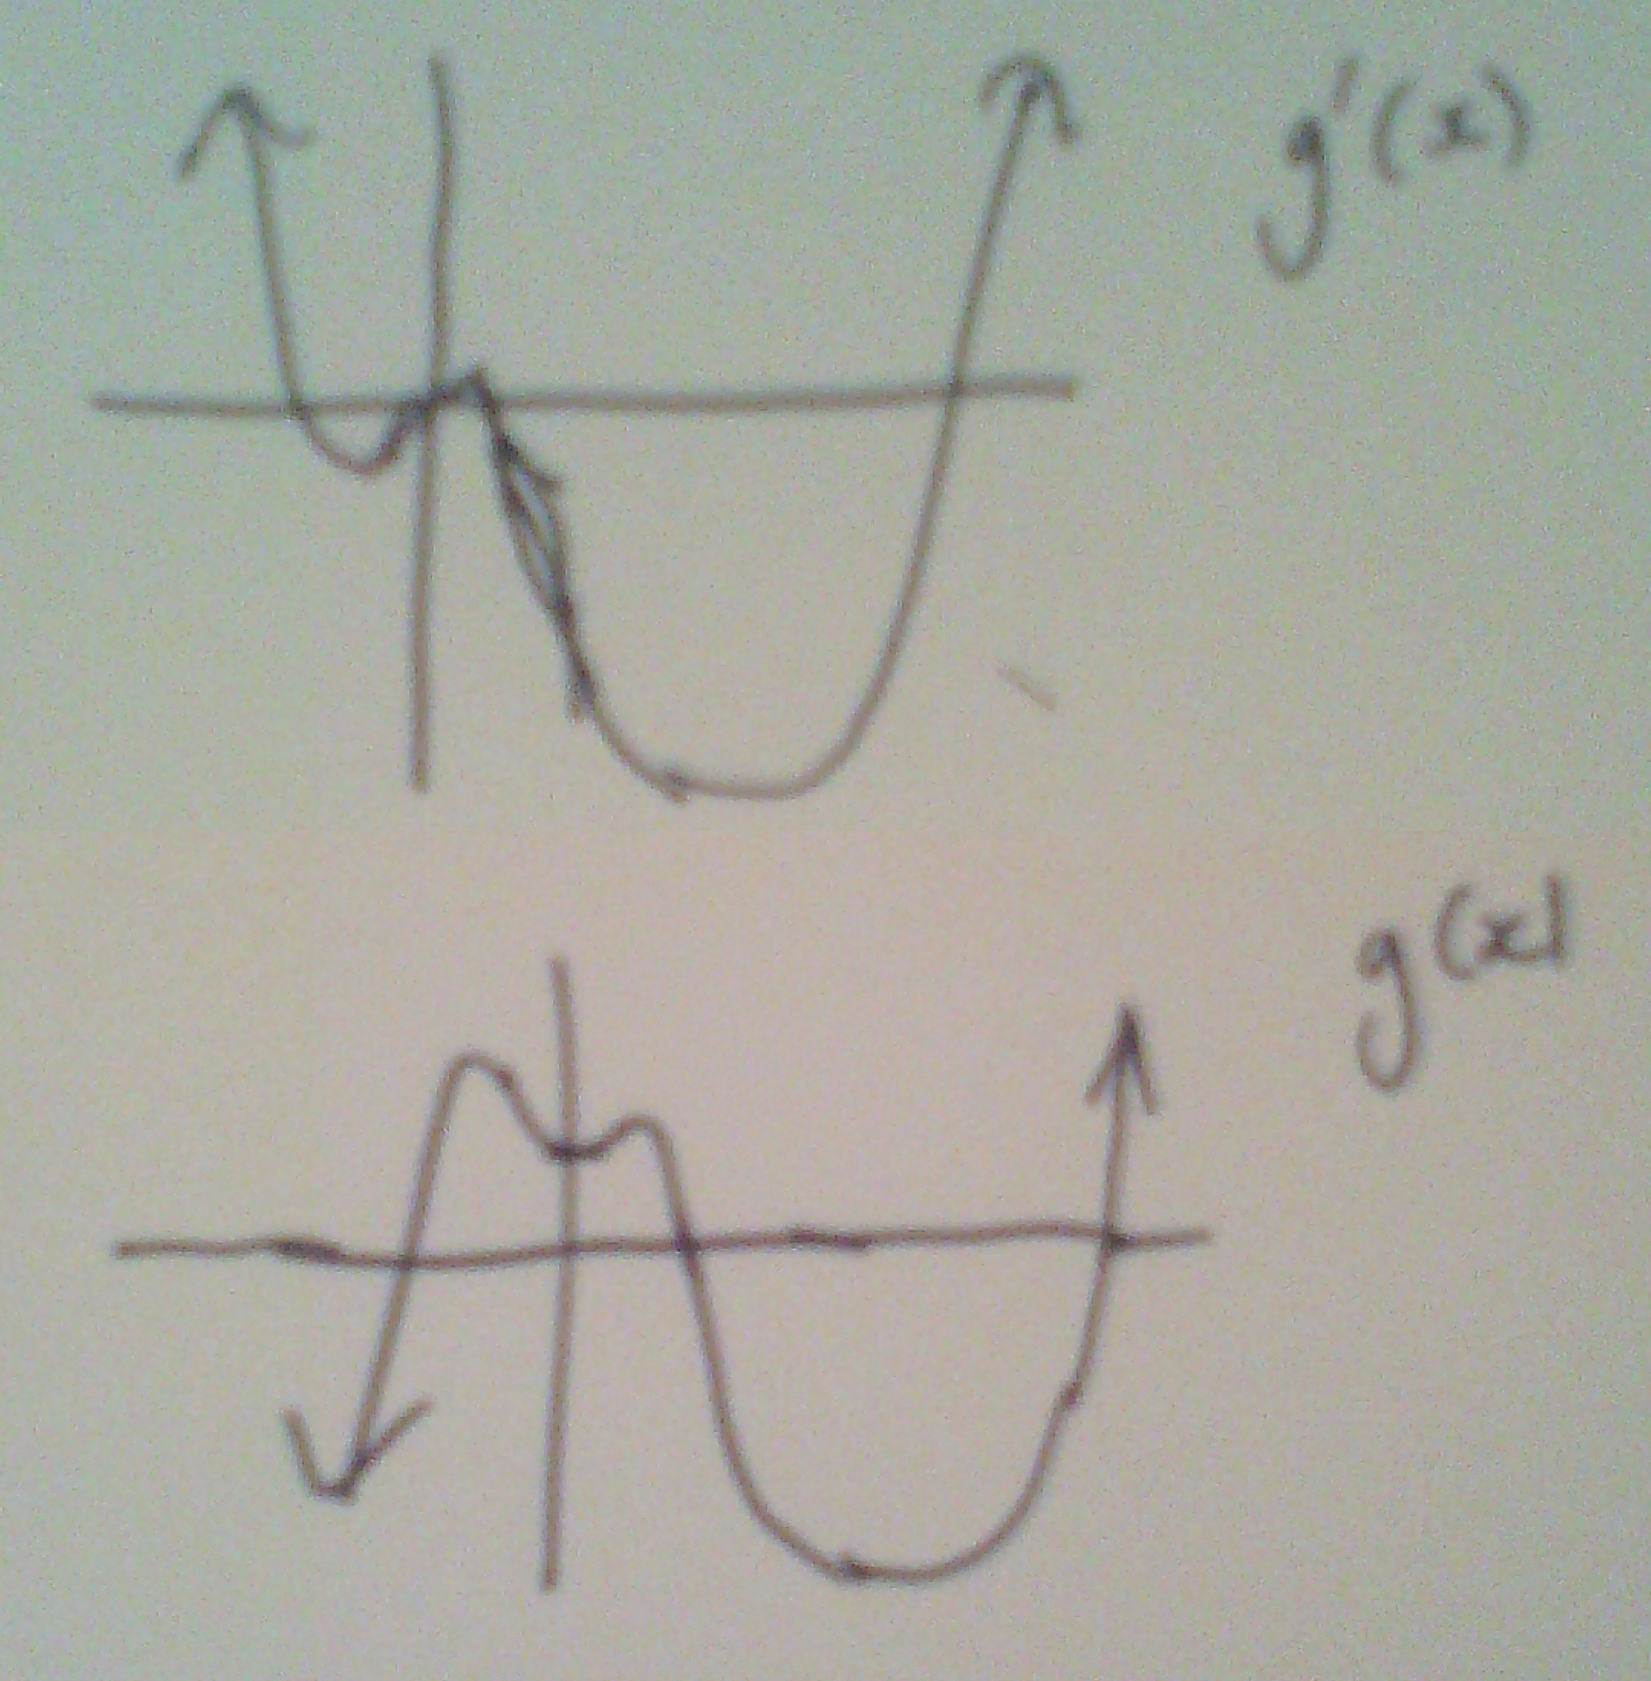
\includegraphics[width=0.3\textwidth]{gofx}
        \end{center}
\end{enumerate}

\subsection*{17. The Fundamental Theorem of Calculus}
\begin{enumerate}
  \item $ \rint^{\pi/4}_0 \sec^2 \theta \dif{\theta} = \eval{[\tan \theta]}_0^{\pi/4} = 1 $.
  \item $ \rint^2_1 f(x) \dif{x} = \rint^3_1 f(x) \dif{x} - \rint^3_2 f(x) \dif{x} = 10 $.
  \item First we find the intersection points; we have $ 6x = x^2 $, so $ x \in \{0, 6\} $. Hence we compute
        \begin{displaymath}
          \rint^6_0 2x - \frac{x^2}{3} \dif{x} = \eval{[x^2 - \frac{x^3}{9}]}_0^6 = 36 - 6^3/9 = 12.
        \end{displaymath}
\end{enumerate}

\subsection*{18. Substitution}
\begin{enumerate}
  \item
    \begin{enumerate}
      \item $ \frac{\csc 3x}{3} + C $.
      \item $ -\frac{\tan 3x^2}{6} + C $.
      \item $ 2\sqrt{x} + 3x - 2\ln x + C $.
      \item $ \frac{\sin^3 x}{3} - \frac{\sin^5 x}{5} + C $.
    \end{enumerate}
  \item Use trig identity: $ 2 \sin 5x \cos 3x = \sin 8x + \sin 2x $. Then
        \begin{displaymath}
          \rint^{\pi/6}_0 \sin 8x + \sin 2x \dif{x} = \eval{\left[-\frac{\cos 8x}{8} - \frac{\cos 2x}{2}\right]}_0^{\pi/6} = 0.4375.
        \end{displaymath}
  \item $ \frac{1}{2} \tan^{-1} x^2 + C $. (Substitute $ u = x^2 $.)
\end{enumerate}

\subsection*{19. Differential Equations}
\begin{enumerate}
  \item
    \begin{enumerate}
      \item $ \rint e^y \dif{y} = \rint e^t \dif{t} $, so $ e^y = e^t + C $ and $ y = \ln (e^t + C) $.
      \item $ \rint \frac{\dif{y}}{y^2} = \rint t \dif{t} $, so $ -\frac{1}{y} = \frac{1}{2} t^2 + \frac{C}{2} $ and $ y = -\frac{2}{t^2 + C} $.
      \item $ \rint \sec^2 y \dif{y} = \rint \dif{t} $, so $ \tan y = t + C $ and $ y = \tan^{-1} (t + C) $.
      \item $ \rint \sin y \dif{y} = \rint -t\cos t \dif{t} $, so $ -\cos y = \cos t - t \sin t - C $ (by the hint) and $ y = \cos^{-1} (t\sin t - \cos t + C) $.
    \end{enumerate}
  \item Using Newton's law of cooling, $ \od{T}{t} = k(T - T_\infty) $ (where $ T_\infty $ is the ambient temperature). Solving this differential
        equation, we find $ \rint \frac{1}{T - T_\infty} \dif{T} = \rint k \dif{t} $ and so $ T = T_0 e^{kt} + T_\infty $. We have $ T_\infty = \SI{30}{\degree} $,
        and $ T_0 = \SI{100}{\degree} $; also, at $ t = 3 $ we have $ T = 70 $ so $ 70 = 100e^{3k} + 30 $; hence $ k = \frac{\ln 0.4}{3} = -0.31 $ and
        by direct substitution $ T = 100e^{-0.31t} + 30 $. Let $ T = 31 $; then $ t = 14.86 $ and so the temperature will drop to \SI{31}{\degree} after
        around fifteen minutes.
  \item
    \begin{enumerate}
      \item We have $ \od{V}{t} = \text{rate in} - \text{rate out} = 3 - kV $. Hence $ \rint \frac{1}{3 - kV} \dif{V} = \rint \dif{t} $, so
            $ -\frac{\ln(3 - kV)}{k} = t + C $ and $ V = \frac{3 - Ke^{-kt}}{k} $. At $ t = 0 $, $ V = 100 $; so $ 100k = (3 - K) $. We also
            have $ kV = 3 $ where $ V = 120 $, so $ k = 1/40 = 0.025 $. Hnce $ 2.5 = 3 - K $ and $ K = 0.5 $. It immediately follows that
            \begin{displaymath}
              V = \frac{3 - 0.5e^{-0.025t}}{0.025}
            \end{displaymath}
            and at $ t = 10 $, $ V = 104 $ litres.
      \item The rate of water flow out is $ kV = 3 - 0.5e^{-0.025t} $, which is always less than 3 (the rate in). In fact, as $ t \to \infty $,
            the volume tends to \SI{120}{\litre} and the rate in tends to equal the rate out.
            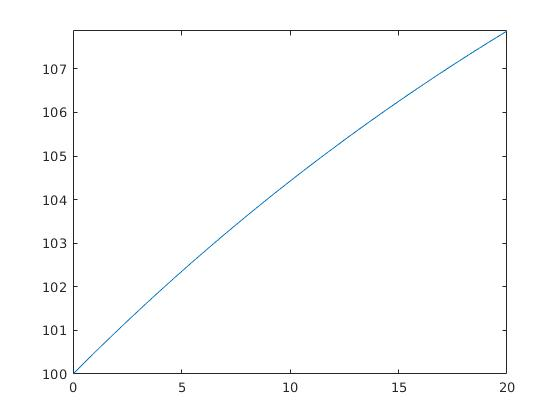
\includegraphics[width=0.3\textwidth]{leakybucket/01}
            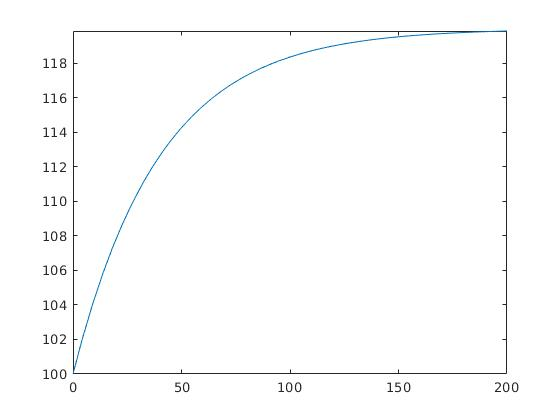
\includegraphics[width=0.3\textwidth]{leakybucket/02}
            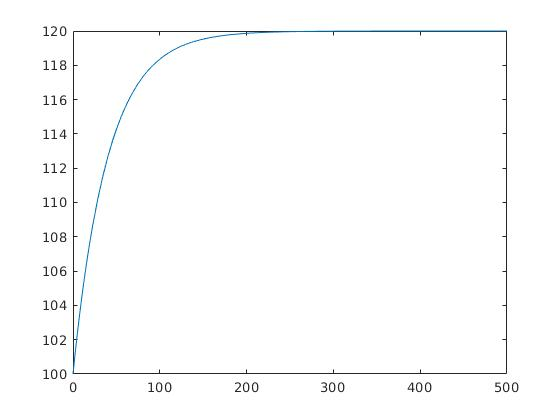
\includegraphics[width=0.3\textwidth]{leakybucket/03}
    \end{enumerate}
\end{enumerate}

\subsection*{20. Partial Fractions}
\begin{enumerate}
  \item
    \begin{enumerate}
      \item
        \begin{align*}
          \rint r \dif{t} &= \rint \frac{\dif{P}}{P(1 - P)} = \\
                          &= \rint \frac{1}{P} + \frac{1}{1 - P} \dif{P}\\
          rt + C &=  \ln\frac{P}{1 - P}\\
          Ke^{rt} &= \frac{P}{1 - P}\\
          \frac{Ke^{rt}}{1 + Ke^{rt}} &= P.
        \end{align*}
      \item It should be clear that as $ t \to \infty $, $ P \to 1 $. (If we look at $ \od{P}{t} = \frac{rP}{P_\infty}(P_\infty - P) $, $ P \to P_\infty $.)

            Green: $ r = K = 1 $; red: $ r = 2 $, $ K = 1 $; blue: $ r = 1 $, $ K = 2 $.
            \begin{center}
              \fbox{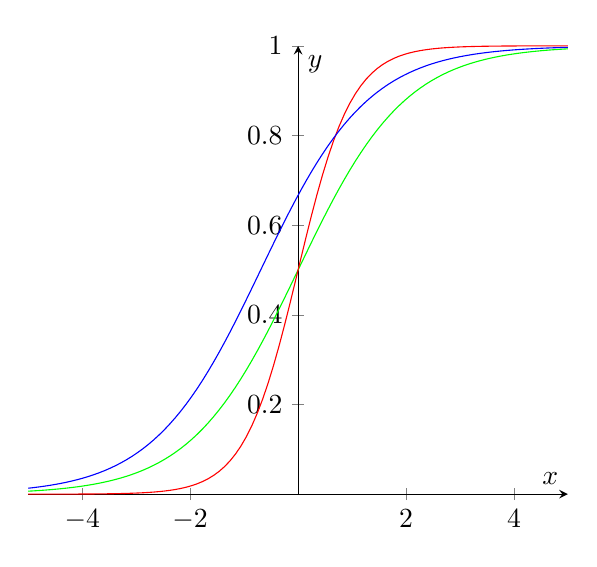
\begin{tikzpicture}
                \begin{axis}[
                  axis lines = center,
                  xlabel = $ x $,
                  ylabel = $ y $
                ]
                  \addplot[domain = -5:5, color = green, samples=100] {(e^x)/(1 + e^x)};
                  \addplot[domain = -5:5, color = red, samples=100] {(e^(2*x))/(1 + e^(2*x))};
                  \addplot[domain = -5:5, color = blue, samples=100] {(2*e^(x))/(1 + 2*e^(x))};
                \end{axis}
              \end{tikzpicture}}
            \end{center}
      \item $ r $ lets us vary how fast the population gets to the maximum. Green: $ r = K = 1 $; red: $ r = 0 $; blue: $ r = -1 $.
            \begin{center}
              \fbox{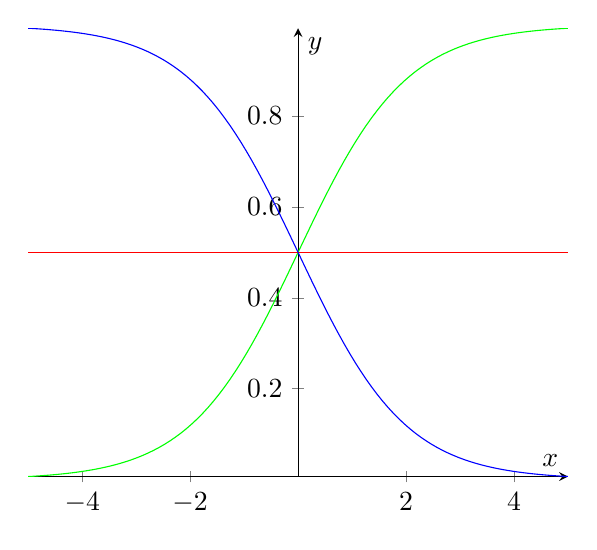
\begin{tikzpicture}
                \begin{axis}[
                  axis lines = center,
                  xlabel = $ x $,
                  ylabel = $ y $
                ]
                  \addplot[domain = -5:5, color = green, samples=100] {(e^x)/(1 + e^x)};
                  \addplot[domain = -5:5, color = red, samples=100] {(e^(0))/(1 + e^(0))};
                  \addplot[domain = -5:5, color = blue, samples=100] {(e^(-x))/(1 + e^(-x))};
                \end{axis}
              \end{tikzpicture}}
            \end{center}
      \item Write it yourself.
    \end{enumerate}
  \item
    \begin{enumerate}
      \item Draw a triangle with angle $ x/2 $, hypotenuse $ \sqrt{1 + t^2} $, adjacent edge $ 1 $, and opposite edge $ t $.
      \item
        \begin{gather*}
          \sin x = 2\sin(x/2)\cos(x/2) = \frac{2t}{1 + t^2}\\
          \cos x = (\cos(x/2))^2 - (\sin(x/2))^2 = \left(\frac{1}{\sqrt{1 + t^2}}\right)^2 - \left(\frac{t}{\sqrt{1 + t^2}}\right)^2
                 = \frac{1 - t^2}{1 + t^2}.
        \end{gather*}
      \item We have $ x = \tan^{-1} 2t $, so the result follows immediately.
      \item
        \begin{enumerate}
          \item Let $ t = \tan(x/2) $. Then, substituting, we have
            \begin{displaymath}
              \rint \frac{1}{1 - \frac{1 - t^2}{1 + t^2}} \cdot \frac{2}{1 + t^2} \dif{t} = \rint \frac{1}{t^2} \dif{t}
                                                                                          = -\frac{1}{t} + C = -\frac{1}{\tan\frac{x}{2}} + C.
            \end{displaymath}
          \item Similarly,
            \begin{align*}
              \rint \frac{1}{3\frac{2t}{1 + t^2} - 4\frac{1 - t^2}{1 + t^2}} \cdot \frac{2}{1 + t^2} \dif{t}
                  &= \rint \frac{1}{3t - 2 + 2t^2} \dif{t} = \rint \frac{1}{(2t - 1)(t + 2)} \dif{t}\\
                  &= \frac{1}{5}\ln\frac{1 - 2t}{t + 2} + C = \frac{1}{5}\ln\frac{1 - 2\tan\frac{x}{2}}{\tan\frac{x}{2} + 2} + C.
            \end{align*}
        \end{enumerate}
    \end{enumerate}
\end{enumerate}

\subsection*{21. Integration by Parts}
\begin{enumerate}
  \item
    \begin{enumerate}
      \item
        \begin{displaymath}
          \rint x \cos 5x \dif{x} = \frac{1}{5} x \sin 5x - \rint \frac{1}{5}\sin 5x \dif{x} = \frac{1}{5}(x\sin 5x + \cos 5x) + C.
        \end{displaymath}
      \item
        \begin{align*}
          \rint \cos x \ln \sin x \dif{x} &= \sin x \ln \sin x - \rint \sin x \frac{\cos x}{\sin x} \dif{x}\\
                                          &= \sin x \ln \sin x - \rint \cos x \dif{x} = \sin x (\ln \sin x - 1) + C.
        \end{align*}
      \item Let $ u = \sqrt{x} $, so $ \dif{x} = 2u \dif{u} $ and our integral becomes
            \begin{displaymath}
              \rint 2u \cos u \dif{u} = 2u\sin u - \rint 2\sin u \dif{u} = 2u \sin u + 2\cos u + C = 2\sqrt{x} \sin \sqrt{x} + 2 \cos \sqrt{x} + C.
            \end{displaymath}
    \end{enumerate}
  \item
    \begin{enumerate}
      \item Let $ u = \theta^2 $, so our integral becomes $ \frac{1}{2} \rint^\pi_{\pi/2}  u \cos u \dif{u} $. From 1(c) above,
            we know that $ \rint u \cos u \dif{u} = u \sin u + \cos u + C $. Hence the required result is
            \begin{displaymath}
              \frac{1}{2} \rint^\pi_{\pi/2}  u \cos u \dif{u} = \frac{1}{2} \eval{\left[u \sin u + \cos u\right]}_{u = \pi/2}^{\pi} = -\frac{1}{2} - \frac{\pi}{4}.
            \end{displaymath}
      \item We use integration by parts twice.
            \begin{align*}
              \rint (x^2 + 1)e^{-x} \dif{x} &= -e^{-x}(x^2 + 1) + \rint 2x e^{-x} \dif{x}\\
                                            &= -e^{-x}(x^2 + 1) - 2xe^{-x} + \rint 2e^{-x} \dif{x}\\
                                            &= -e^{-x}(x^2 + 1) - 2xe^{-x} -2e^{-x} + C.
            \end{align*}
            Hence the result we are looking for is $ 3 - 6e^{-1} $.
    \end{enumerate}
  \item
    \begin{enumerate}
      \item Apply integration by parts to $ \rint 1 \cdot (\ln x)^n \dif{x} $ by integrating $ 1 $ and differentiating $ (\ln x)^n $.
      \item Applying (a), we find
            \begin{align*}
              \rint (\ln x)^3 \dif{x} &= x(\ln x)^3 - \rint (\ln x)^{2} \dif{x}\\
                                      &= x(\ln x)^3 - (x(\ln x)^2 - \rint \ln x \dif{x})\\
                                      &= x(\ln x)^3 - (x(\ln x)^2 - (x\ln x - x))\\
                                      &= x(\ln x)^3 - x(\ln x)^2 + x\ln x - x.
            \end{align*}
    \end{enumerate}
\end{enumerate}

\subsection*{22. Lengths, Volumes, and Areas}
\begin{enumerate}
  \item We simply calculate the relevant integral:
        \begin{displaymath}
          \pi \rint_1^2 x^{-2} \dif{x} = \pi [(-2^{-1}) - (-1^{-1})] = \frac{\pi}{2}.
        \end{displaymath}
  \item Calculating the surface area:
        \begin{align*}
          2\pi \rint_0^\pi \sin x \sqrt{1 - \cos^2 x} \dif{x} &= 2\pi \rint_0^\pi \sin^2 x \dif{x}\\
                                                              &= \pi \eval{\left[ x - \sin 2x \right]}_0^\pi\\
                                                              &= \pi^2
        \end{align*}
        So the radius of the equivalent circle is $ \sqrt{\pi} $.
  \item Summing along the axis from base to point, each slice has an area $ \left(\frac{L}{H}{x}\right)^2 = \frac{L^2}{H^2}x^2 $;
        hence the total volume is
        \begin{displaymath}
          V = \rint_0^H \frac{L^2}{H^2}x^2 \dif{x} = \frac{1}{3} L^2 H.
        \end{displaymath}
  \item We have $ r = a(1 - \cos \theta) $ so $ \od{r}{\theta} = a\sin \theta $. Hence:
        \begin{align*}
          S &= \rint^{2\pi}_0 \sqrt{a^2(1-\cos\theta)^2 + a^2\sin^2 \theta} \dif{\theta}\\
            &= \rint^{2\pi}_0 \sqrt{a^2 - 2a^2 \cos \theta + a^2(\sin^2 \theta + \cos^2 \theta)} \dif{\theta}\\
            &= a\sqrt{2} \rint^{2\pi}_0 \sqrt{1-\cos\theta} \dif{\theta}.
        \end{align*}
        We turn our attention, then, to the integral $ \rint \sqrt{1-\cos \theta} \dif{\theta} $. Let $ u = 1 - \cos \theta $;
        then $ \dif{u} = \sin \theta \dif{\theta} $; but $ \sin \cos^{-1} (1 - u) = \sqrt{2u - u^2} $ (this can be verified by drawing
        a suitable triangle). Hence $ \dif{u} = \sqrt{2u - u^2} \dif{\theta} $, and
        \begin{align*}
          \rint \sqrt{1-\cos \theta} \dif{\theta} &= \rint \frac{\sqrt{u}}{\sqrt{2u - u^2}} \dif{u}\\
                                                  &= \rint \frac{1}{\sqrt{2 - u}}\\
                                                  &= -2\sqrt{2 - u} + C\\
                                                  &= -2\sqrt{1 + \cos \theta} + C.
        \end{align*}
        Therefore (and changing our integral to double the integral from $ 0 $ to $ \pi $ to avoid the problem of having a closed loop),
        \begin{align*}
          S &= 2a\sqrt{2} \rint^{\pi}_0 \sqrt{1-\cos\theta} \dif{\theta}\\
            &= 2a\sqrt{2} \eval{\left[ -2\sqrt{1 + \cos \theta} \right]}_0^{\pi}\\
            &= 2a\sqrt{2} \left[(-2\sqrt{1 + \cos \pi}) - (-2\sqrt{1 + \cos 0})\right]\\
            &= 2a\sqrt{2} \left[(-2\sqrt{0}) - (-2\sqrt{2})\right]\\
            &= 2a\sqrt{2} \times 2\sqrt{2} = 8a.
        \end{align*}
\end{enumerate}

\subsection*{23. Trigonometric Substitution}
\emph{These ones are tedious and can be checked by the computer, so I have not written full answers for all of them.}
\begin{enumerate}
  \item Let $ x = 2 \tan \theta $, so $ \dif{x} = 2\sec^2 \theta $:
        \begin{displaymath}
          \rint \frac{2\sec^2 \theta}{\sqrt{x^2 + 4}} \dif{x} = \rint \frac{\sec^2 \theta}{\sqrt{1 + \tan^2 x}} \dif{x} = \rint \sec \theta \dif{x}
            = \ln\left( \sqrt{\left(\frac{x}{2}\right)^2 + 1} + \frac{x}{2} \right) + C.
        \end{displaymath}
  \item First, let $ u = x^7 $ so $ \dif{u} = 7x^6 \dif{x} $ and our integral becomes
        \begin{displaymath}
          \frac{1}{7} \rint \frac{\dif{u}}{\sqrt{1 - u^2}} = \frac{1}{14} \ln \frac{1 + u}{1 - u} + C = \frac{1}{14} \ln \frac{1 + x^7}{1 - x^7} + C.
        \end{displaymath}
  \item Use $ x = \frac{2}{5} \sec \theta $.
  \item Use $ x = \frac{2}{3} \sin \theta $.
  \item Use $ x = \frac{1}{6} \tan \theta $ and simplify.
  \item Use integration by parts; the resulting integral $ - \frac{\ln x}{4x^4} + \rint \frac{\dif{x}}{4x^5} $ is much simpler.
  \item Use partial fractions.
\end{enumerate}

\subsection*{24. Kinematics}
\begin{enumerate}
  \item
    \begin{enumerate}
      \item $ v = \od{h}{t} = 122.5 - 9.8t $, so the initial velocity of the flare is \SI{122.5}{\metre\per\second}.
      \item Zero.
      \item When $ v = 0 $, $ t = 12 $ and the height at this time is around 764 metres.
    \end{enumerate}
  \item Let $ x $ be the distance from the point on the beach directly away from B. Then the total distance travelled
        is simply $ D = \sqrt{600^2 + x^2} + \sqrt{800^2 + (1200-x)^2} $; taking the derivative:
        \begin{displaymath}
          \od{D}{x} = \frac{x}{\sqrt{600^2 + x^2}} - \frac{1200 - x}{\sqrt{800^2 + (1200 - x)^2}}
        \end{displaymath}
        Setting to zero, we have
        \begin{gather*}
          x\sqrt{800^2 + (1200 - x)^2} = (1200 - x)\sqrt{600^2 + x^2}\\
          800^2 x^2 + (1200 - x)^2 x^2 = (1200 - x)^2 (600^2 + x^2)\\
          0 =  1200^2 600^2 - 600^2 2400x + (600^2 - 800^2) x^2\\
          x \in \{ -3600, 3600/7 \}.
        \end{gather*}
        Since $ x \geq 0 $, $ x = 3600/7 \approx 514 $. The total distance travelled is therefore around 1844 metres. By graphing $ D $ versus $ x $,
        we see that this is indeed the required medium:
        \begin{center}
          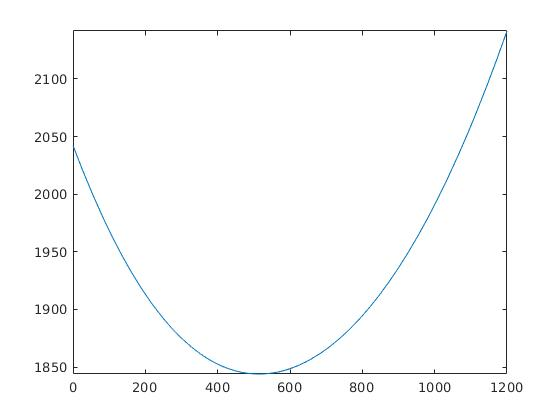
\includegraphics[width=0.4\textwidth]{swamp}
        \end{center}
\end{enumerate}

\subsection*{25. Integration Revision}
\begin{enumerate}
  \item
    \begin{enumerate}
      \item $ \rint^2_1 \sin x \dif{x} = \eval{[-\cos x]}_1^2 = \cos 1 - \cos 2 $.
      \item $ \rint \frac{u^2 + 1}{u^3 + 3u} = \frac{1}{3} \ln (u^3 + 3u) + C $.
      \item $ \rint^{\pi/6}_0 \tan x \dif{x} = \eval{[\ln \sec x]}_0^{\pi/6} \approx 0.1438 $.
    \end{enumerate}
  \item We have $ \od{y}{x} = \frac{3x^2 + 4x - 4}{2y - 4} $, so $ \rint 2y - 4 \dif{y} = \rint 3x^2 + 4x - 4 \dif{x} $.
        Hence $ y^2 - 4y = x^3 + 2x^2 - 4x + C $; we also have $ C = -2 $, so $ y^2 - 4y = x^3 + 2x - 4x - 2 $. We are
        trying to find $ y $ if $ x = 2 $; so $ y^2 - 4y = 8 + 4 - 4 - 2 = 6 $. Solving $ y^2 - 4y - 6 = 0 $, we find
        $ y = \frac{4 \pm \sqrt{38}}{2} $.
  \item
    \begin{enumerate}
      \item Let $ t = a \tan \theta $. Then:
            \begin{align*}
              \rint \frac{a^3}{t^2 + a^2} \dif{t} &= \rint \frac{a^4 \sec^2 \theta}{a^2 \tan^2 + a^2} \dif{\theta}\\
                                                  &= \rint \frac{a^2 \sec^2 \theta}{\sec^2 \theta} \dif{\theta}\\
                                                  &= a^2 \theta = a^2 \tan^{-1} \left(\frac{t}{a}\right);
            \end{align*}
            hence $ \omega(a,x) = a^2 \tan^{-1} \left(\frac{x}{a}\right) $.
      \item It follows that $ \omega(2,2) = 4\tan^{-1} 1 = \pi $.
      \item We wish to find $ x $ such that $ \pi = 3 \tan^{-1} \left(\frac{x}{\sqrt{3}}\right) $;
            in other words, $ x = \sqrt{3} \tan\left(\frac{\pi}{3}\right) = 3 $.
    \end{enumerate}
  \item Note first that $ \rint^{\pi/2}_{-\pi/2} \sin^5 x \dif{x} = 0 $ since $ \sin^5 $ is odd. Then, we argue as follows:
        \begin{align*}
          \rint \cos^5 x \dif{x} &= \rint \cos x (1 - \sin^2 x)^2 \dif{x}\\
                                 &= \rint (1 - t^2)^2 \dif{t} \qquad\text{($ t = \sin x $)}\\
                                 &= \rint 1 - 2t^2 + t^4 \dif{t}\\
                                 &= t - \frac{2}{3}t^3 + \frac{t^5}{5} + C\\
                                 &= \sin x - \frac{2}{3} \sin^3 x + \frac{1}{5} \sin^5 x + C.
        \end{align*}
        Hence
        \begin{displaymath}
          \rint^{\pi/2}_{-\pi/2} \sin^5 x \dif{x} = (\sin \frac{\pi}{2} - \frac{2}{3} \sin^3 \frac{\pi}{2} + \frac{1}{5} \sin^5 \frac{\pi}{2}) - (\sin \frac{-\pi}{2} - \frac{2}{3} \sin^3 \frac{-\pi}{2} + \frac{1}{5} \sin^5 \frac{-\pi}{2}).
        \end{displaymath}
        But $ \sin (\pi/2) = 1 $; so we have $ (1 - \frac{2}{3} + \frac{1}{5}) - (-1 + \frac{2}{3} - \frac{1}{5}) = 2(1 - \frac{2}{3} + \frac{1}{5}) = \frac{16}{15} $.
\end{enumerate}

\end{document}
